\documentclass[xcolor=svgnames]{beamer}
%\documentclass[xcolor=svgnames, handout]{beamer}

%\includeonlyframes{current}

\usepackage[utf8]    {inputenc}
\usepackage[T1]      {fontenc}
\usepackage[english] {babel}

\usepackage{amsmath,amsfonts,graphicx}
\usepackage{beamerleanprogress}
\usepackage{xcolor}
\usepackage{soul}
%\usepackage{verbatim}
\usepackage{multicol}
\usepackage{tikz} 
\usepackage[export]{adjustbox}

\hypersetup{colorlinks,urlcolor=blue}


\definecolor{iyellow}{RGB}{255, 162, 23}
\definecolor{sgreen}{RGB}{118, 191, 138}

\newcommand{\yellow}[1]{\textcolor{iyellow}{#1}}
\newcommand{\red}[1]{\textcolor{red}{#1}}
\newcommand{\green}[1]{\textcolor{ForestGreen}{#1}}
\newcommand{\blue}[1]{{\textcolor{blue}{#1}}}
\newcommand{\orange}[1]{{\textcolor{orange}{#1}}}
\newcommand{\bblue}[1]{\textcolor{SteelBlue!90!gray}{#1}} % beamer blue

\newcommand{\eol}{\\[1em]\pause}
\newcommand{\nl}{\\[1em]}
\newcommand{\define}[1]{\textbf{\textcolor{orange}{#1}}}
\newcommand{\answer}[1]{\textit{\textbf{\textcolor{iyellow}{#1}}}}
\newcommand{\command}[1]{\texttt{\textbf{\textcolor{DarkMagenta}{#1}}}}
\newcommand{\ipic}[2]{\includegraphics[width={#2}\textwidth]{#1}}
\newcommand{\cell}[1]{{\sf \textbf{\textcolor{DarkMagenta}{#1}}}}
\newcommand{\ra}{$\rightarrow$}

% timed answer
\newcommand{\tans}[2]{\textbf<#1>{\textit<#1>{{\color<#1>{iyellow}{#2}}}}}

\newcommand{\ft}[1]{\frametitle{#1}}

% for straight quotes in verbatim:
\usepackage{upquote,textcomp}

\usepackage[T1]{fontenc}
\usepackage[utf8]{inputenc}
\usepackage{tikz}
\usetikzlibrary{shadows}

\newcommand*\keystroke[1]{%
  \tikz[baseline=(key.base)]
    \node[%
      draw,
      fill=white,
      drop shadow={shadow xshift=0.25ex,shadow yshift=-0.25ex,fill=black,opacity=0.75},
      rectangle,
      rounded corners=2pt,
      inner sep=1pt,
      line width=0.5pt,
      font=\scriptsize\sffamily
    ](key) {#1\strut}
  ;
}

\title
  [Data 301 Data Analytics\hspace{2em}]
  {Data 301 Data Analytics\\
  Open Data}

\author
  [Dr.\ Irene Vrbik]
  {Dr.\ Irene Vrbik}

\date
  {Term 1, 2018}

\institute
  {University of British Columbia Okanagan \newline irene.vrbik@ubc.ca}


\graphicspath{{img/}}

\begin{document}

\maketitle

\setbeamersize{description width=0.57cm} % to have less indent with the description environment



\begin{frame}
  {What is open data?}

  \begin{itemize}
  \item \define{Open Data} is the movement to make data freely available to all with no restrictions on use or copyright.\nl

\item Governments have been major supporters and providers of open data as data collected by governments is primarily done to benefit its citizens.\nl

\item Corporations and other organizations are both producers and consumers of open data.

  \end{itemize}
\end{frame}


\begin{frame}{Open data in Canada}
\begin{itemize}
\item Federal, provincial, and local governments have all been involved in the open data movement.\nl

\item Canadian Federal government: \url{http://open.canada.ca/en}
\begin{itemize}
\item How to use: \url{http://open.canada.ca/en/working-data}
\item Statistics Canada: \url{http://www.statcan.gc.ca/eng/rdc/data}\nl
\end{itemize}

\item British Columbia government: \url{http://www.data.gov.bc.ca/}\nl

\item City of Kelowna: \url{http://opendata.kelowna.ca/}
%\url{https://www.kelowna.ca/city-services/city-maps-open-data/open-data-catalogue}
\end{itemize}
\end{frame}


\begin{frame}{Open Data in Canada}
\begin{center}
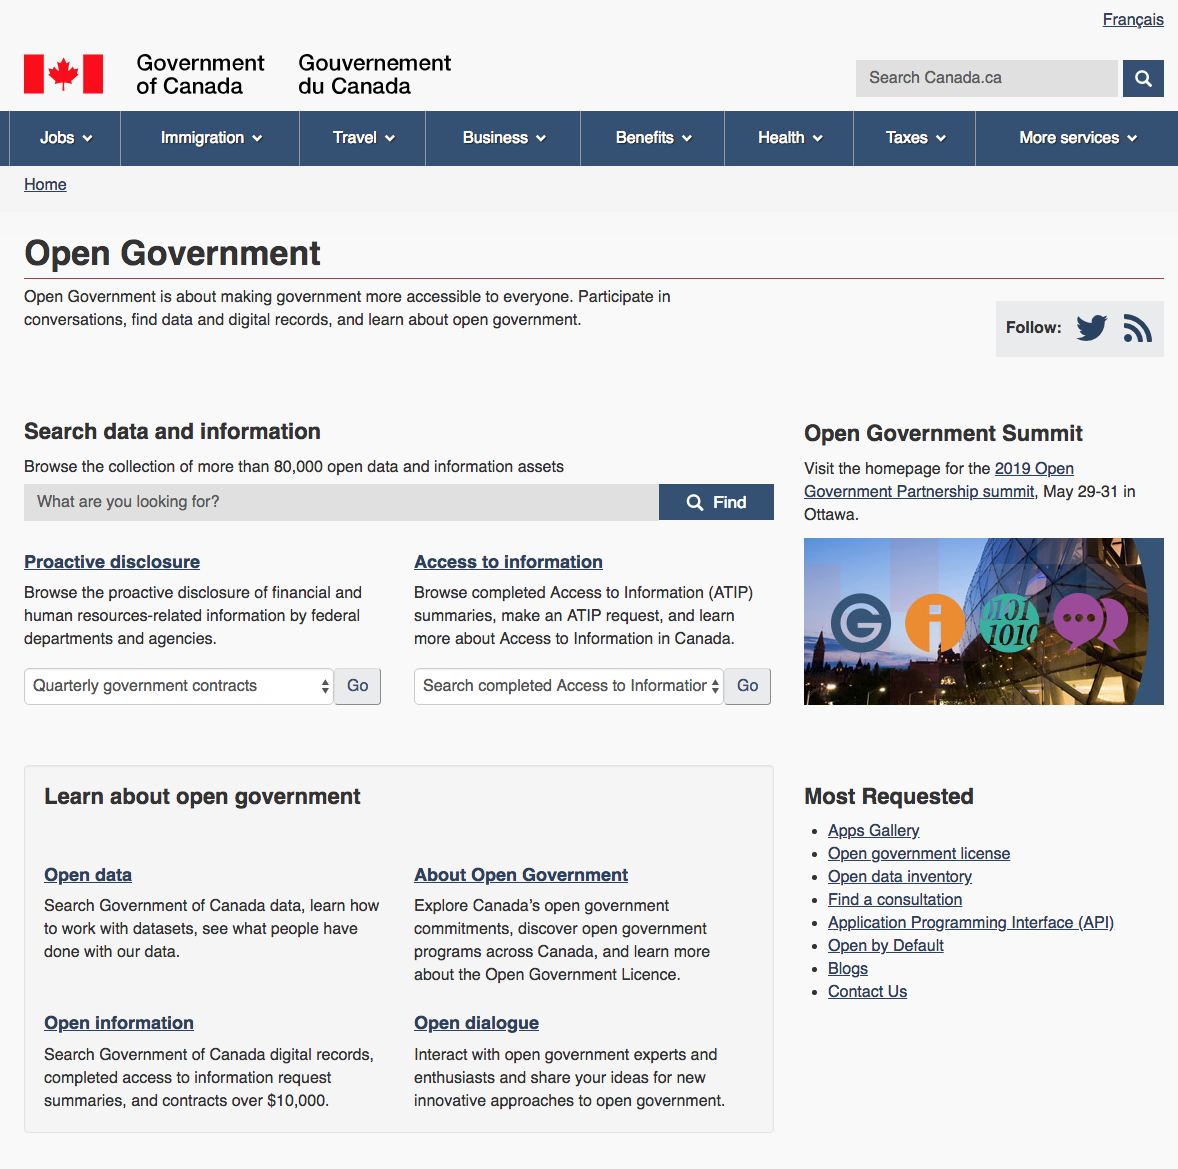
\includegraphics[width=0.9\textwidth]{img/gov}
\end{center}
\end{frame}

\begin{frame}{Open Data in BC}{Example: MSP Blue Book}
\begin{itemize}
\item For example, the BC Medical Services Plan's (MSP) allows access to the annual financial statements including a detailed listing of total annual payments to all practitioners and organizations. \nl
\item Payments for 2010-11 to 2015-16 are provided \href{https://catalogue.data.gov.bc.ca/dataset/msp-blue-book}{here} and statements for the last 10 years are currently posted on the Ministry website.\nl
\item Published by the Ministry of Health - Medical Services 
\item Licensed under Open Government Licence - British Columbia
\end{itemize}
\end{frame}


\begin{frame}{Open Data in BC}{Example: MSP Blue Book}
\begin{center}
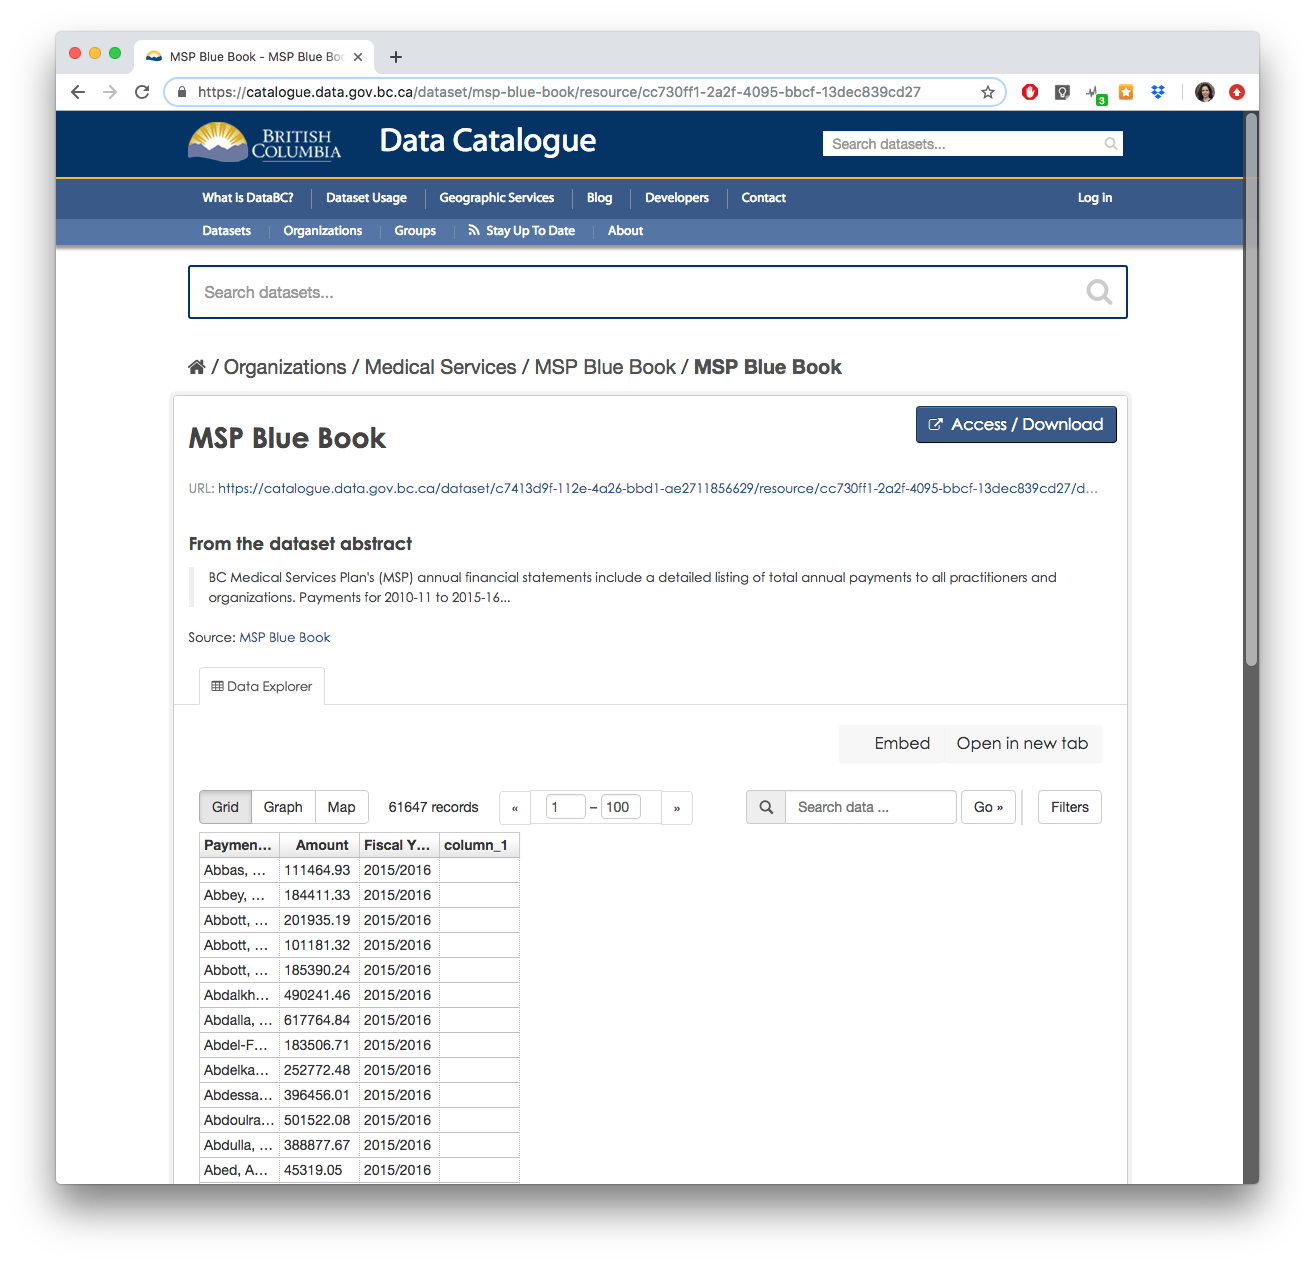
\includegraphics[width=0.9\textwidth]{img/MSPBlueBook}
\end{center}
\end{frame}



\begin{frame}{Open Data in BC}{Example: DriveBC}
\begin{itemize}
\item DriveBC is the British Columbia Ministry of Transportation and Infrastructure's traveller information system. 
\item \href{https://catalogue.data.gov.bc.ca/dataset/drivebc}{This website} provides timely road condition and incident information for the provincial highway system, motorists can decide when to travel and what route to take.
\item  This information is updated at regular intervals and as highway conditions change. 
\item Traveller information is provided only for provincially-managed transportation routes in British Columbia.
\item  Federal, municipal, forest service and industrial resource roads are not considered part of the provincial highway system, and therefore are not reported on through DriveBC.
\item Published by the Ministry of Transportation and Infrastructure - Business Management Services 
\item Licensed under Access Only
\end{itemize}
\end{frame}

\begin{frame}{Open Data in Kelowna}
\begin{center}
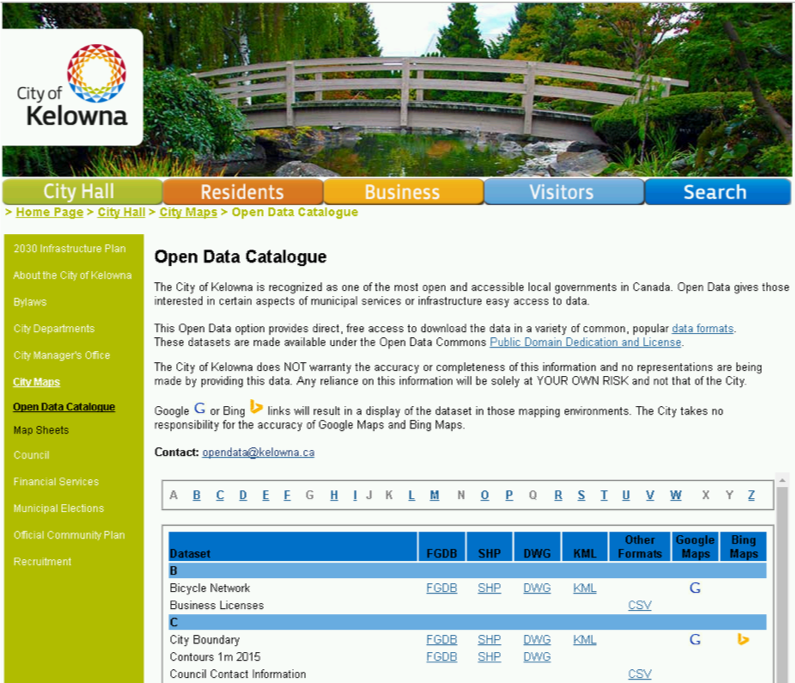
\includegraphics[width=0.9\textwidth]{img/kewl}
\end{center}
\end{frame}


\begin{frame}{Open Data in United States}
\begin{itemize}
\item United States government: \url{https://www.data.gov/}\nl

\item Individual states have their own open data sites as well:
\begin{itemize}
\item Example: Washington state: \url{https://data.wa.gov/}
\end{itemize}
\end{itemize}
\end{frame}


\begin{frame}{United States: Data.gov}
\begin{center}
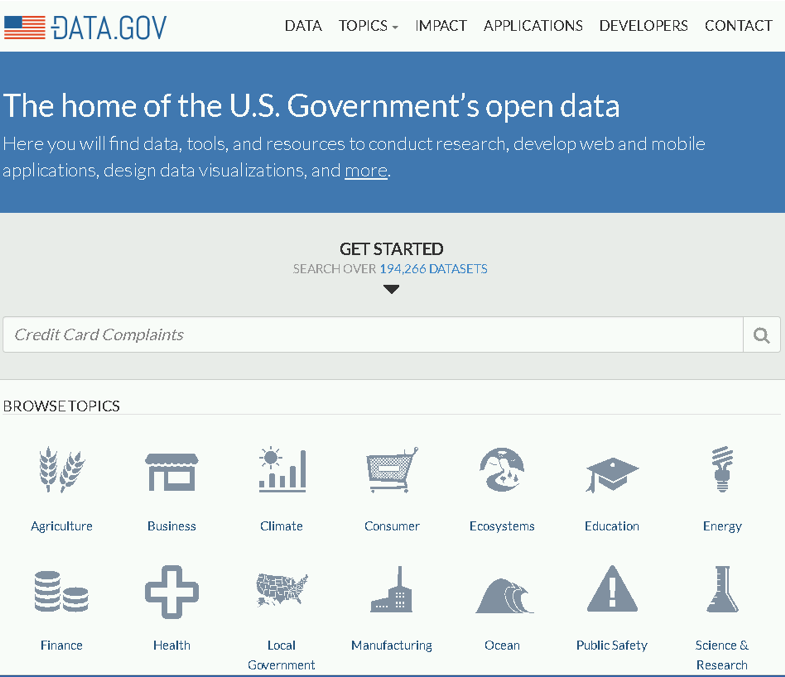
\includegraphics[width=0.9\textwidth]{img/us}
\end{center}
\end{frame}


\begin{frame}{Open Data Worldwide}
\begin{itemize}
\item UK: \url{http://data.gov.uk}\nl

\item The World Bank: \url{http://data.worldbank.org/}
\begin{itemize}
\item Financial information and statistics\nl
\end{itemize}

\item  United Nations: \url{http://data.un.org/}\nl

\item OECD (Organisation for Economic Co-operation and Development): \url{https://data.oecd.org/}

\end{itemize}
\end{frame}


\begin{frame}{Open Data Aggregation}
\begin{itemize}
\item There are many sites that aggregate open data sets (and some data sets for a cost). A Canadian based site is \href{http://www.quandl.com}{Quandl}.\nl

\item \href{https://www.kaggle.com/datasets}{Kaggle} provides many data sets and competitions and techniques for data analytics and machine learning.  \nl

\item More recently, Google has released a search engine called \href{https://toolbox.google.com/datasetsearch}{Dataset Search} for finding data sets. 
\begin{itemize}
\item provides easier access to millions of datasets across thousands of data repositories on the web.
\end{itemize}

\end{itemize}
\end{frame}


\begin{frame}{Open Data from Companies}
Many companies either have public data or application programming interfaces (APIs) that allow people to use their data.
\begin{itemize}
\item Google: \href{https://www.google.com/publicdata/directory}{public data explorer} and \href{https://developers.google.com/maps}{Google Maps API}
\item Facebook: \url{https://developers.facebook.com/} (API)
\item reddit: \url{https://www.reddit.com/dev/api} (API)
\item Twitter: \url{https://dev.twitter.com/rest/public} (API)
\item Amazon: \url{https://aws.amazon.com/public-data-sets/} (public data sets) and \url{https://developer.amazon.com/} (API for developers)
\item Best Buy: \url{https://developer.bestbuy.com/} (API)
\end{itemize}
\end{frame}


\begin{frame}{Your turn}
\begin{itemize}
\item Explore the federal, provincial, and City of Kelowna data sets to discover ``something interesting".\nl %Report to your neighbors and to the class.

\item From any Canadian government open data site, retrieve a data set and analyze and visualize it using one of our tools: Excel, R, Python, Tableau.

\end{itemize}
\end{frame}


\begin{frame}{Open Data for Researcher}
\begin{itemize}
\item Increasingly publicly funded researchers are responsible for making their data sets, procedures, and results available to the public (and other researchers).
\begin{itemize}
\item Canadian researchers funded by \href{http://www.nserc-crsng.gc.ca/NSERC-CRSNG/policies-politiques/OpenAccessFAQ-LibreAccesFAQ\_eng.asp}{NSERC}, SSHRC, CIHR must make their publications freely available within 12 months of publication.
\item Researchers in bioinformatics and other fields must make their data sets publically available in a database or repository.\nl
\end{itemize}

\item  Researchers benefit by having access to public data sets and data sets of other researchers, but there is also a challenge as producing data sets (and perhaps commercializing results) may restrict open access.

\end{itemize}
\end{frame}




\begin{frame}{Open Data Biology/Bioinformatics}
Huge number of databases with most related to  \href{http://www.ncbi.nlm.nih.gov/}{NCBI} but distributed world-wide.
\begin{center}
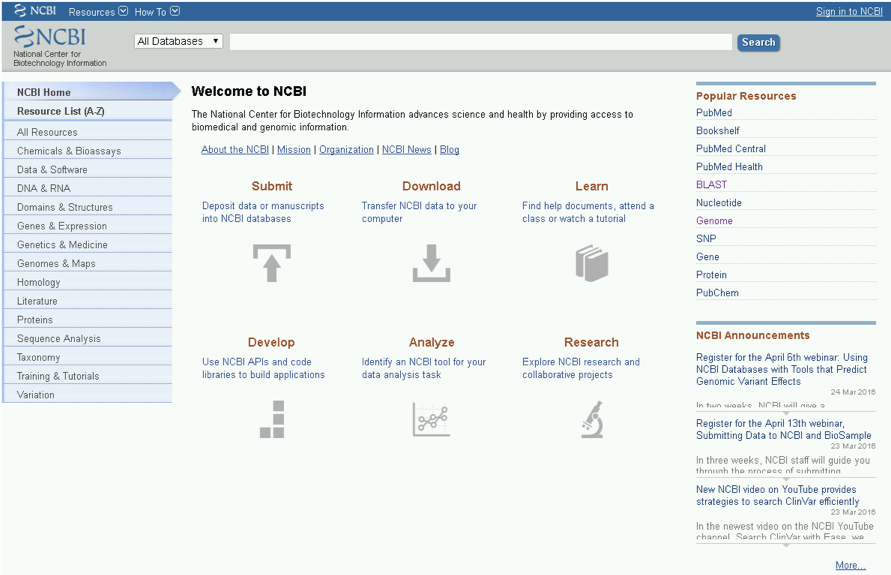
\includegraphics[width=0.9\textwidth]{img/ncbi}
\end{center}

\end{frame}

\begin{frame}{Open Data in Chemistry}
\begin{itemize}
\item ChEMBL (\url{https://www.ebi.ac.uk/chembl/}) stores structures and properties of pharmacologically active molecules.
\begin{itemize}
\item Over 1.5 million compounds.\nl
\end{itemize}


\item  SureChEMBL (\url{https://www.surechembl.org}) is a database extracted automatically from patent applications.
\begin{itemize}
\item  Growing at 80,000 compounds a month and has 16 million compounds from over 13 million annotated patents.\nl
\end{itemize}

\item  ChemSpider (\url{http://www.chemspider.com/}) is a free chemical structure database containing over 43 million structures.
\begin{itemize}
\item  Supported and hosted by Royal Society of Chemistry.
\end{itemize}
\end{itemize}
\end{frame}

\begin{frame}{Open Data in Computer Science}
\begin{itemize}
\item Computer scientists in various fields create standardized data sets for experimentation and research.\nl

\begin{itemize}
\item  Databases: Standard performance benchmarks such as TPC (\url{www.tpc.org}).\medskip
\item Machine learning/data mining: UCI ML repository \url{http://archive.ics.uci.edu/ml/} \medskip
\item Game path finding: \url{http://www.movingai.com/benchmarks/}\medskip
\end{itemize}


\end{itemize}
\end{frame}

\begin{frame}{Open Data in Earth/Environment Science}
\begin{itemize}
\item Climate Change Data Portal: \url{http://sdwebx.worldbank.org/climateportal/}\medskip
\item National Climatic Data Center: \url{https://www.ncdc.noaa.gov/cdo-web/}\medskip
\item National Geographic Data Center: \url{http://www.nodc.noaa.gov/submit/}\medskip
\item Polar Data Catalog: \url{https://www.polardata.ca/}\medskip
\end{itemize}
\begin{center}
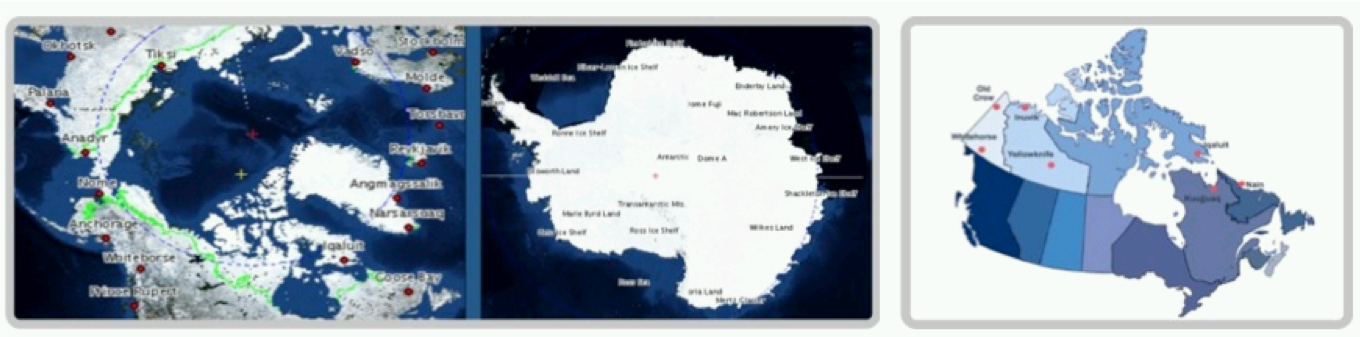
\includegraphics[width=0.9\textwidth]{img/earth}
\end{center}

\end{frame}

\begin{frame}{Open Data in Physics}
Modern physics produces a HUGE amount in data in experiments like astronomical observations and the Large Hadron Collider (\href{https://home.cern/science/accelerators/large-hadron-collider}{LHC}; the worlds largest particle accelorator).
\begin{itemize}
\item New research systems developed to handle the large amount of data produced.
\item \href{https://home.cern/}{CERN} (The European Organization for Nuclear Research) open data portal: \url{http://opendata.cern.ch/}
\item Data produced is tens of petabytes/year. Large distributed computing of 170 facilities in 36 countries.\nl
\end{itemize}

Astronomy:
\begin{itemize}
\item Canadian Astronomy Data Centre: \url{http://www3.cadc-ccda.hia-iha.nrc-cnrc.gc.ca/cadc/}
\item National Space Science Data Center: \url{http://nssdc.gsfc.nasa.gov/}
\end{itemize}
\end{frame}



\begin{frame}{Open Data in Psychology and Social Sciences}
Archaeology: 
\begin{itemize}
\item Archaeology Data Service: http://archaeologydataservice.ac.uk/
\item Many museums have online exhibits and open data.\nl
\end{itemize}

Psychology:
\begin{itemize}
\item Journals increasing requiring open data sets.
\item List of open data sites at: \url{http://guides.library.ucla.edu/c.php?g=180221\&p=1188487}
\end{itemize}


History	
\begin{itemize}
\item Digital Archive Database Project (UBC): \url{http://dadp.ok.ubc.ca}
\end{itemize}
\end{frame}


\begin{frame}{Github}
\begin{itemize}
\item \href{https://github.com/}{Github} is another service that provides a platform for publishing open (as well as private data).\nl
\item GitHub also provides a %\href{https://github.com/awesomedata/awesome-public-datasets}{repository}  for datasets
\href{https://github.com/collections/open-data}{collection} of open data\nl
\item {Canada} has an \href{https://github.com/open-data}{Open Government} initiative that is housed on GitHub.\nl
\item There is a also a \href{https://usopendata.org/}{US Open Data} project on \href{https://github.com/opendata}{Github}
\end{itemize}

\end{frame}


\begin{frame}{Google Analytics}
\begin{itemize}
\item \define{Google Analytics} is an analysis service for tracking, optimizing, and understanding user interaction with a web site/service.\nl

\item Using \href{https://analytics.google.com/analytics/web/provision/?authuser=0\#/provision}{Google analytics} is important for all business, but especially web companies, that rely on users interacting with their site to generate revenue and sales.\nl

\item Google analytics helps identify and improve content to make it more accessible to potential customers.
\begin{itemize}
\item Google has a series of online \href{https://analytics.google.com/analytics/academy/}{courses}.
\end{itemize}

%Very important skill set for business owners and managers.

\end{itemize}
\end{frame}

\begin{frame}{Google Ads}
\href{https://ads.google.com/intl/en\_CA/home/}{Google Ads} (previous Google AdWords) is a service to provide advertisements during searches and as display advertisements on web sites and in apps. 

\begin{itemize}
\item Companies bid on keywords and display opportunities that are presented by Google and affiliated sites.\nl
\item In 2017, the primary source of revenue from Google AdWords. \href{https://www.investopedia.com/articles/investing/020515/business-google.asp}{Source}.\nl
\item With great power comes great responsibility:
\begin{itemize}
\item Google CEO Sundar Pichai \href{https://www.youtube.com/watch?v=8qS7eyUo\_uk}{testifies before Congress} about data breaches, misinformation campaigns, and concerns about working with China. \nl
\end{itemize}
\end{itemize}
\end{frame}

\begin{frame}{Google Ads}


Terminology:
\begin{description}
\item[Ad Impression] - display of an advertisement. Pricing in cost-per-thousand impressions or cost per mille (CPM).
\item[Click through] - user clicks on an advertisement (and directly to new location)
\item[Click through rate] - fraction of impressions that are clicked on
\item[Pay-per-click (PPC)] - companies are billed on each click of an advertisement. The pricing depends on the bid amount and the desirability of the ad location.
\end{description}

\end{frame}



\begin{frame}{Conclusion}
\begin{itemize}
\item Open Data is the movement to make data freely available to all with no restrictions on use or copyright.\medskip
\item Open data has been widely supported by governments and companies wishing to engage users (and developers) with their services.\medskip
\item Data analysts should use open data to help with their analysis whenever available.\medskip
\item Researchers are often responsible for making their publications and data available in an open fashion.\medskip
\item Google provides services for analytics and advertising that are valuable to understand as a business or site looking for user traffic.
\end{itemize}
\end{frame}

\begin{frame}{Objectives}
\begin{itemize}
\item Define open data and explain the motivations for making data ``open''.\nl
\item List some of the governments and organizations that provide data in an open fashion.\nl
\item Use open data sets when applicable when performing data analysis.\nl
%\item Explain the role of Google Analytics and Google Ads. 
%\item Compare and contrast what these two services provide.
\end{itemize}
\end{frame}



\end{document}

